% !Mode:: "TeX:UTF-8"
\documentclass[12pt,a4paper]{article}

%%%%%%%%------------------------------------------------------------------------
%%%% 日常所用宏包

%% 控制页边距
% 如果是beamer文档类, 则不用geometry
\makeatletter
\@ifclassloaded{beamer}{}{\usepackage[top=2.5cm, bottom=2.5cm, left=2.5cm, right=2.5cm]{geometry}}
\makeatother

%% 控制项目列表
\usepackage{enumerate}

%% 多栏显示
\usepackage{multicol}

%% 算法环境
\usepackage{algorithm}  
\usepackage{algorithmic} 
\usepackage{float} 

%% 网址引用
\usepackage{url}

%% 控制矩阵行距
\renewcommand\arraystretch{1.4}

%% hyperref宏包,生成可定位点击的超链接,并且会生成pdf书签
\makeatletter
\@ifclassloaded{beamer}{
\usepackage{hyperref}
\usepackage{ragged2e} % 对齐
}{
\usepackage[%
    pdfstartview=FitH,%
    CJKbookmarks=true,%
    bookmarks=true,%
    bookmarksnumbered=true,%
    bookmarksopen=true,%
    colorlinks=true,%
    citecolor=blue,%
    linkcolor=blue,%
    anchorcolor=green,%
    urlcolor=blue%
]{hyperref}
}
\makeatother



\makeatletter % 如果是 beamer 不需要下面两个包
\@ifclassloaded{beamer}{
\mode<presentation>
{
} 
}{
%% 控制标题
\usepackage{titlesec}
%% 控制目录
\usepackage{titletoc}
}
\makeatother

%% 控制表格样式
\usepackage{booktabs}

%% 控制字体大小
\usepackage{type1cm}

%% 首行缩进,用\noindent取消某段缩进
\usepackage{indentfirst}

%% 支持彩色文本、底色、文本框等
\usepackage{color,xcolor}

%% AMS LaTeX宏包: http://zzg34b.w3.c361.com/package/maths.htm#amssymb
\usepackage{amsmath,amssymb}
%% 多个图形并排
\usepackage{subfig}
%%%% 基本插图方法
%% 图形宏包
\usepackage{graphicx}
\newcommand{\red}[1]{\textcolor{red}{#1}}
\newcommand{\blue}[1]{\structure{#1}}
\newcommand{\brown}[1]{\textcolor{brown}{#1}}
\newcommand{\green}[1]{\textcolor{green}{#1}}


%%%% 基本插图方法结束

%%%% pgf/tikz绘图宏包设置
\usepackage{pgf,tikz}
\usetikzlibrary{shapes,automata,snakes,backgrounds,arrows}
\usetikzlibrary{mindmap}
%% 可以直接在latex文档中使用graphviz/dot语言,
%% 也可以用dot2tex工具将dot文件转换成tex文件再include进来
%% \usepackage[shell,pgf,outputdir={docgraphs/}]{dot2texi}
%%%% pgf/tikz设置结束


\makeatletter % 如果是 beamer 不需要下面两个包
\@ifclassloaded{beamer}{

}{
%%%% fancyhdr设置页眉页脚
%% 页眉页脚宏包
\usepackage{fancyhdr}
%% 页眉页脚风格
\pagestyle{plain}
}

%% 有时会出现\headheight too small的warning
\setlength{\headheight}{15pt}

%% 清空当前页眉页脚的默认设置
%\fancyhf{}
%%%% fancyhdr设置结束


\makeatletter % 对 beamer 要重新设置
\@ifclassloaded{beamer}{

}{
%%%% 设置listings宏包用来粘贴源代码
%% 方便粘贴源代码,部分代码高亮功能
\usepackage{listings}

%% 设置listings宏包的一些全局样式
%% 参考http://hi.baidu.com/shawpinlee/blog/item/9ec431cbae28e41cbe09e6e4.html
\lstset{
showstringspaces=false,              %% 设定是否显示代码之间的空格符号
numbers=left,                        %% 在左边显示行号
numberstyle=\tiny,                   %% 设定行号字体的大小
basicstyle=\footnotesize,                    %% 设定字体大小\tiny, \small, \Large等等
keywordstyle=\color{blue!70}, commentstyle=\color{red!50!green!50!blue!50},
                                     %% 关键字高亮
frame=shadowbox,                     %% 给代码加框
rulesepcolor=\color{red!20!green!20!blue!20},
escapechar=`,                        %% 中文逃逸字符,用于中英混排
xleftmargin=2em,xrightmargin=2em, aboveskip=1em,
breaklines,                          %% 这条命令可以让LaTeX自动将长的代码行换行排版
extendedchars=false                  %% 这一条命令可以解决代码跨页时,章节标题,页眉等汉字不显示的问题
}}
\makeatother
%%%% listings宏包设置结束


%%%% 附录设置
\makeatletter % 对 beamer 要重新设置
\@ifclassloaded{beamer}{

}{
\usepackage[title,titletoc,header]{appendix}
}
\makeatother
%%%% 附录设置结束


%%%% 日常宏包设置结束
%%%%%%%%------------------------------------------------------------------------


%%%%%%%%------------------------------------------------------------------------
%%%% 英文字体设置结束
%% 这里可以加入自己的英文字体设置
%%%%%%%%------------------------------------------------------------------------

%%%%%%%%------------------------------------------------------------------------
%%%% 设置常用字体字号,与MS Word相对应

%% 一号, 1.4倍行距
\newcommand{\yihao}{\fontsize{26pt}{36pt}\selectfont}
%% 二号, 1.25倍行距
\newcommand{\erhao}{\fontsize{22pt}{28pt}\selectfont}
%% 小二, 单倍行距
\newcommand{\xiaoer}{\fontsize{18pt}{18pt}\selectfont}
%% 三号, 1.5倍行距
\newcommand{\sanhao}{\fontsize{16pt}{24pt}\selectfont}
%% 小三, 1.5倍行距
\newcommand{\xiaosan}{\fontsize{15pt}{22pt}\selectfont}
%% 四号, 1.5倍行距
\newcommand{\sihao}{\fontsize{14pt}{21pt}\selectfont}
%% 半四, 1.5倍行距
\newcommand{\bansi}{\fontsize{13pt}{19.5pt}\selectfont}
%% 小四, 1.5倍行距
\newcommand{\xiaosi}{\fontsize{12pt}{18pt}\selectfont}
%% 大五, 单倍行距
\newcommand{\dawu}{\fontsize{11pt}{11pt}\selectfont}
%% 五号, 单倍行距
\newcommand{\wuhao}{\fontsize{10.5pt}{10.5pt}\selectfont}
%%%%%%%%------------------------------------------------------------------------


%% 设定段间距
\setlength{\parskip}{0.5\baselineskip}

%% 设定行距
\linespread{1}


%% 设定正文字体大小
% \renewcommand{\normalsize}{\sihao}

%制作水印
\RequirePackage{draftcopy}
\draftcopyName{XTUMESH}{100}
\draftcopySetGrey{0.90}
\draftcopyPageTransform{40 rotate}
\draftcopyPageX{350}
\draftcopyPageY{80}

%%%% 个性设置结束
%%%%%%%%------------------------------------------------------------------------


%%%%%%%%------------------------------------------------------------------------
%%%% bibtex设置

%% 设定参考文献显示风格
% 下面是几种常见的样式
% * plain: 按字母的顺序排列,比较次序为作者、年度和标题
% * unsrt: 样式同plain,只是按照引用的先后排序
% * alpha: 用作者名首字母+年份后两位作标号,以字母顺序排序
% * abbrv: 类似plain,将月份全拼改为缩写,更显紧凑
% * apalike: 美国心理学学会期刊样式, 引用样式 [Tailper and Zang, 2006]

\makeatletter
\@ifclassloaded{beamer}{
\bibliographystyle{apalike}
}{
\bibliographystyle{unsrt}
}
\makeatother


%%%% bibtex设置结束
%%%%%%%%------------------------------------------------------------------------

%%%%%%%%------------------------------------------------------------------------
%%%% xeCJK相关宏包

\usepackage{xltxtra,fontspec,xunicode}
\usepackage[slantfont, boldfont]{xeCJK} 
\usepackage{bm}

\setlength{\parindent}{2em}%中文缩进两个汉字位

%% 针对中文进行断行
\XeTeXlinebreaklocale "zh"             

%% 给予TeX断行一定自由度
\XeTeXlinebreakskip = 0pt plus 1pt minus 0.1pt

%%%% xeCJK设置结束                                       
%%%%%%%%------------------------------------------------------------------------

%%%%%%%%------------------------------------------------------------------------
%%%% xeCJK字体设置

%% 设置中文标点样式,支持quanjiao、banjiao、kaiming等多种方式
\punctstyle{kaiming}                                        
                                                     
%% 设置缺省中文字体
%\setCJKmainfont[BoldFont={Adobe Heiti Std}, ItalicFont={Adobe Kaiti Std}]{Adobe Song Std}   
\setCJKmainfont{SimSun}
%% 设置中文无衬线字体
%\setCJKsansfont[BoldFont={Adobe Heiti Std}]{Adobe Kaiti Std}  
%% 设置等宽字体
%\setCJKmonofont{Adobe Heiti Std}                            

%% 英文衬线字体
\setmainfont{DejaVu Serif}                                  
%% 英文等宽字体
\setmonofont{DejaVu Sans Mono}                              
%% 英文无衬线字体
\setsansfont{DejaVu Sans}                                   

%% 定义新字体
\setCJKfamilyfont{song}{Adobe Song Std}                     
\setCJKfamilyfont{kai}{Adobe Kaiti Std}
\setCJKfamilyfont{hei}{Adobe Heiti Std}
\setCJKfamilyfont{fangsong}{Adobe Fangsong Std}
\setCJKfamilyfont{lisu}{LiSu}
\setCJKfamilyfont{youyuan}{YouYuan}

%% 自定义宋体
\newcommand{\song}{\CJKfamily{song}}                       
%% 自定义楷体
\newcommand{\kai}{\CJKfamily{kai}}                         
%% 自定义黑体
\newcommand{\hei}{\CJKfamily{hei}}                         
%% 自定义仿宋体
\newcommand{\fangsong}{\CJKfamily{fangsong}}               
%% 自定义隶书
\newcommand{\lisu}{\CJKfamily{lisu}}                       
%% 自定义幼圆
\newcommand{\youyuan}{\CJKfamily{youyuan}}                 

%%%% xeCJK字体设置结束
%%%%%%%%------------------------------------------------------------------------

%%%%%%%%------------------------------------------------------------------------
%%%% 一些关于中文文档的重定义
\newcommand{\chntoday}{\number\year\,年\,\number\month\,月\,\number\day\,日}
%% 数学公式定理的重定义

%% 中文破折号,据说来自清华模板
\newcommand{\pozhehao}{\kern0.3ex\rule[0.8ex]{2em}{0.1ex}\kern0.3ex}

\newtheorem{example}{例}                                   
\newtheorem{theorem}{定理}[section]                         
\newtheorem{definition}{定义}
\newtheorem{axiom}{公理}
\newtheorem{property}{性质}
\newtheorem{proposition}{命题}
\newtheorem{lemma}{引理}
\newtheorem{corollary}{推论}
\newtheorem{remark}{注解}
\newtheorem{condition}{条件}
\newtheorem{conclusion}{结论}
\newtheorem{assumption}{假设}

\makeatletter %
\@ifclassloaded{beamer}{

}{
%% 章节等名称重定义
\renewcommand{\contentsname}{目录}     
\renewcommand{\indexname}{索引}
\renewcommand{\listfigurename}{插图目录}
\renewcommand{\listtablename}{表格目录}
\renewcommand{\appendixname}{附录}
\renewcommand{\appendixpagename}{附录}
\renewcommand{\appendixtocname}{附录}
%% 设置chapter、section与subsection的格式
\titleformat{\chapter}{\centering\huge}{第\thechapter{}章}{1em}{\textbf}
\titleformat{\section}{\centering\sihao}{\thesection}{1em}{\textbf}
\titleformat{\subsection}{\xiaosi}{\thesubsection}{1em}{\textbf}
\titleformat{\subsubsection}{\xiaosi}{\thesubsubsection}{1em}{\textbf}

\@ifclassloaded{book}{

}{
\renewcommand{\abstractname}{摘要}
}
}
\makeatother

\renewcommand{\figurename}{图}
\renewcommand{\tablename}{表}

\makeatletter
\@ifclassloaded{book}{
\renewcommand{\bibname}{参考文献}
}{
\renewcommand{\refname}{参考文献} 
}
\makeatother

\floatname{algorithm}{算法}
\renewcommand{\algorithmicrequire}{\textbf{输入:}}
\renewcommand{\algorithmicensure}{\textbf{输出:}}

%%%% 中文重定义结束
%%%%%%%%------------------------------------------------------------------------



\title{时变偏微分方程的隐式显式方法}
\author{刘江刚}
\date{\chntoday}

\begin{document}
\maketitle
\newpage
摘要~~隐式显式(IMEX)格式已被广泛使用,尤其是与谱方法结合,用于扩散对流型空间离散偏微分方程(PDEs)的时间积分。通常,隐式格式用于扩散项,显式格式用于对流项。反应扩散问题也可以用这种方式近似。在这些工作中,我们系统地分析了这些格式的性能,提出了改进的新格式,并且特别关注它们在快速多重网格算法和谱方法的$\textcolor{red}{\text{混叠}}$减少的背景下的相对性能。(在统计、信号处理和相关领域中,混叠是指取样信号被还原成连续信号时产生彼此交叠而失真的现象。当混叠发生时,原始信号无法从取样信号还原)。

对于原型线性对流扩散方程,进行了一阶、二阶、三阶和四阶多步IMEX格式的稳定性分析。确定了允许大的时间步长用于各种问题并且产生高频误差模式的适当衰减的稳定格式。数值实验表明,当使用有限差分空间离散化的多重网格计算时,高频模式的弱衰减会导致最细的网格上的额外迭代,并且当使用谱配置法进行空间离散时,会导致混叠。当出现这种情况时,不建议使用弱阻尼格式,例如Crank-Nicolson与二阶Adams-Bashforth的流行组合,并提出更好的替代方案。
\section{模型}
考虑一个时间相关的PDE,其中空间导数已经通过中心有限差分或谱方法离散化,这就产生了一个常微分方程系统,它通常具有以下这种形式
\begin{equation}
u'=f(u)+\nu g(u)
\end{equation}
其中$\nu$是非负参数。这里我们对$\nu g(u)$进行隐式处理,$f(u)$进行显式处理,这就产生了IMEX格式。

迄今为止最流行的IMEX格式是用于显式(“对流”)项的二阶Adams-Bashforth和用于隐式(“扩散”)项的Crank-Nicolson的组合。应用于(1)将得出:
\begin{equation}
\frac{u^{n+1}-u^n}{k}=\frac{3}{2}f(u^n)-\frac{1}{2}f(u^{n-1})+\frac{\nu}{2}[g(u^{n+1})+g(u^n)]
\end{equation}
其中$k$是离散时间步长,$u^n$是$u(kn)$的数值近似。
\section{一阶隐式显式格式}
对于(1)一个参数的一阶IMEX格式可以写成
\begin{equation}
u^{n+1}-u^n=kf(u^n)+\nu k[(1-\gamma)g(u^n)+\gamma g(u^{n+1})]
\end{equation}
我们限制$0\le\gamma\le 1$为了防止大的截断误差。

我们选择$\gamma=0$得到向前Euler格式
\begin{equation}
u^{n+1}-u^n=kf(u^n)+\nu kg(u^n)
\end{equation}

当$f=0$时,选择$\gamma=\frac{1}{2}$得到二阶Crank-Nicolson格式。

另一种可能是对$g$采用向后Euler格式,对$f$采用向前Euler格式。选择$\gamma=1$得到
\begin{equation}
u^{n+1}-u^n=kf(u^n)+\nu kg(u^{n+1})
\end{equation}
诸如(5)的IMEX格式,将后向微分公式(BDF)应用于离散化$g$,并且将$f$外推到时间步长$(n+1)$将被称为半隐BDF(SBDF)格式。
\section{二阶隐式显式格式}
\begin{equation}
\begin{aligned}
\frac{1}{k}&\left[\left(\gamma+\frac{1}{2}\right)u^{n+1}-2\gamma u^n+\left(\gamma-\frac{1}{2}\right)u^{n-1}\right]=(\gamma+1)f(u^n)-\gamma f(u^{n-1})\\
&+\nu\left[\left(\gamma+\frac{c}{2}\right)g(u^{n+1})+(1-\gamma-c)g(u^n)+\frac{c}{2}g(u^{n-1})\right]
\end{aligned}
\end{equation}
选择$(\gamma,c)=(\frac{1}{2},0)$将得到流行的格式(2)
\begin{equation}
\frac{1}{k}[u^{n+1}-u^n]=\frac{3}{2}f(u^n)-\frac{1}{2}f(u^{n-1})+\frac{\nu}{2}[g(u^{n+1})+g(u^n)]
\end{equation}
因为它对隐式项应用了Crank-Nicolson格式,对显式项应用了Adams-Bashforth格式,这个格式被称为CNAB。当$c=\frac{1}{8}$时,我们证明了$\gamma=\frac{1}{2}$最好的渐进衰减性质,我们将得到以下格式
\begin{equation}
\frac{1}{k}[u^{n+1}-u^n]=\frac{3}{2}f(u^n)-\frac{1}{2}f(u^{n-1})+\nu\left[\frac{9}{16}g(u^{n+1})+\frac{3}{8}g(u^n)+\frac{1}{16}g(u^{n-1})\right]
\end{equation}
因为它跟CNAB格式很相似,所以这个格式被称为修正的CNAB(MCNAB),和CNAB相比,MCNAB需要额外计算和存储$g(u^{n-1})$。

在(6)中我们选择$(\gamma,c)=(0,1)$,我们获得了另一种应用于谱方法的格式
\begin{equation}
\frac{1}{2k}[u^{n+1}-u^{n-1}]=f(u^n)+\frac{\nu}{2}[g(u^{n+1})+g(u^{n-1})]
\end{equation}
这个格式显式项采用了蛙跳格式,隐式项采用了类似于Crank-Nicolson格式,我们称这个格式为CNLF(Crank-Nicolson,leap frog)。

最后我们选择$(\gamma,c)=(1,0)$,我们得到
\begin{equation}
\frac{1}{2k}[3u^{n+1}-4u^n+u^{n-1}]=2f(u^n)-f(u^{n-1})+\nu g(u^{n+1})
\end{equation}
因为该方案以时间步长$(n+1)$为中心,所以它被称为SBDF。

我们可以从$\alpha-\beta$平面中的稳定性区域获得进一步的信息,这些图显示在Fig2-5中,Fig2显示了CNLF的区域。如果$k<\frac{h}{a}$则该格式对于所有$\nu\le 0$都是稳定的。这种时间步长的限制是我们不希望的,因为它可以应用到更大的$\nu$和更小的$h$。此外,当$\alpha\rightarrow-\infty$时,高频模式的衰减很弱,趋向于1。 CNLF与其他$\gamma=0$二阶方法相比,表明CNLF在这些方法中产生最大的稳定区域。

Fig3显示了CNAB的区域,对于较大的$\nu$和较小的$h$,该方法具有合理的时间步长限制。 然而,它在$\beta-$轴附近不稳定。当$\alpha\rightarrow-\infty$时,它也受到高频模式衰减的影响,趋向于1。使用MCNAB,取$(\gamma,c)=(\frac{1}{2},\frac{1}{8})$,这种衰减趋向于$\frac{1}{3}$这是一个显著的改进。见Fig4。

Fig5显示了SBDF的区域,当$\nu$大且$h$小时,该方法具有最好的时间步长限制。当$\alpha\rightarrow-\infty$时,高频模式的衰减很强,趋向于0。然而,该方法对于小的$|\alpha|$具有最严格的时间步长限制。
\begin{figure}[H]
\centering
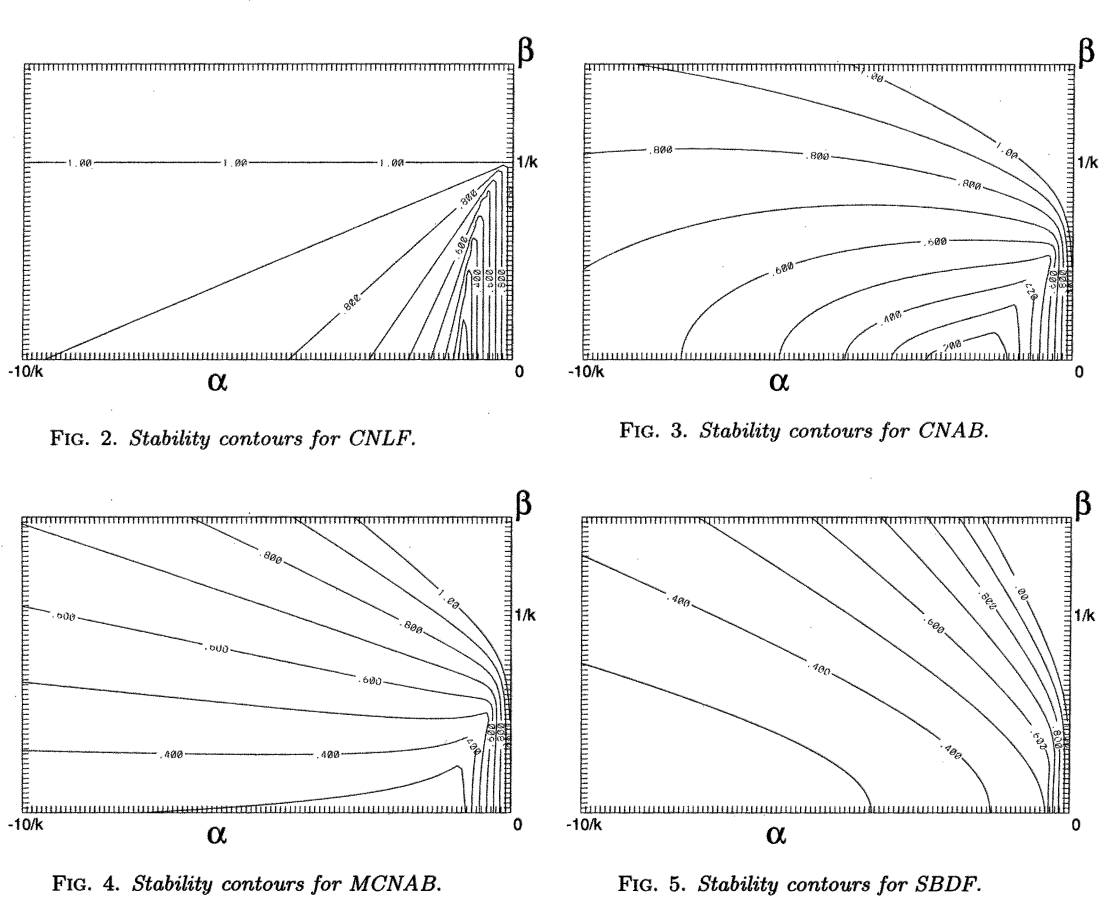
\includegraphics[scale=0.4]{./figures/Figure_1.png}
\end{figure}
定义网格雷诺数
\begin{equation*}
R\equiv\frac{ah}{\nu}
\end{equation*}
在Figs6-8中,我们绘制了各种$\gamma$和$c$的理论时间步长限制。 从这些图中可以看出,当$R<2$时,增加$\gamma$允许更大的稳定时间步长。当$R>2$时,情况$c=1-\gamma$还具有减少$\gamma$允许更大时间步长的特性。Figs6-8表明,对于$R<2$,使用SBDF可以应用最大时间步长,对于$R>2$,使用CNLF可以应用最大时间步长。当离散扩散项时,该结果相应选择SBDF,当离散对流项时,该结果相应选择CNAB。从这个角度来看,当$R\approx 2$时,CNAB更有竞争力。
\begin{figure}[H]
\centering
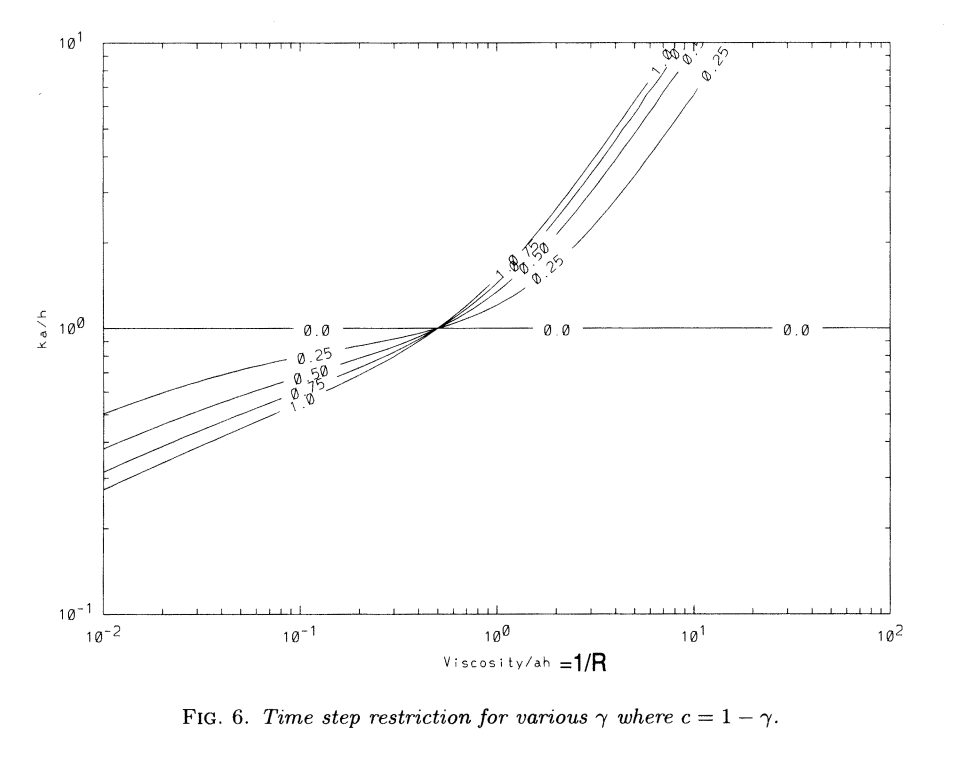
\includegraphics[scale=0.4]{./figures/Figure_2.png}
\end{figure}
\begin{figure}[H]
\centering
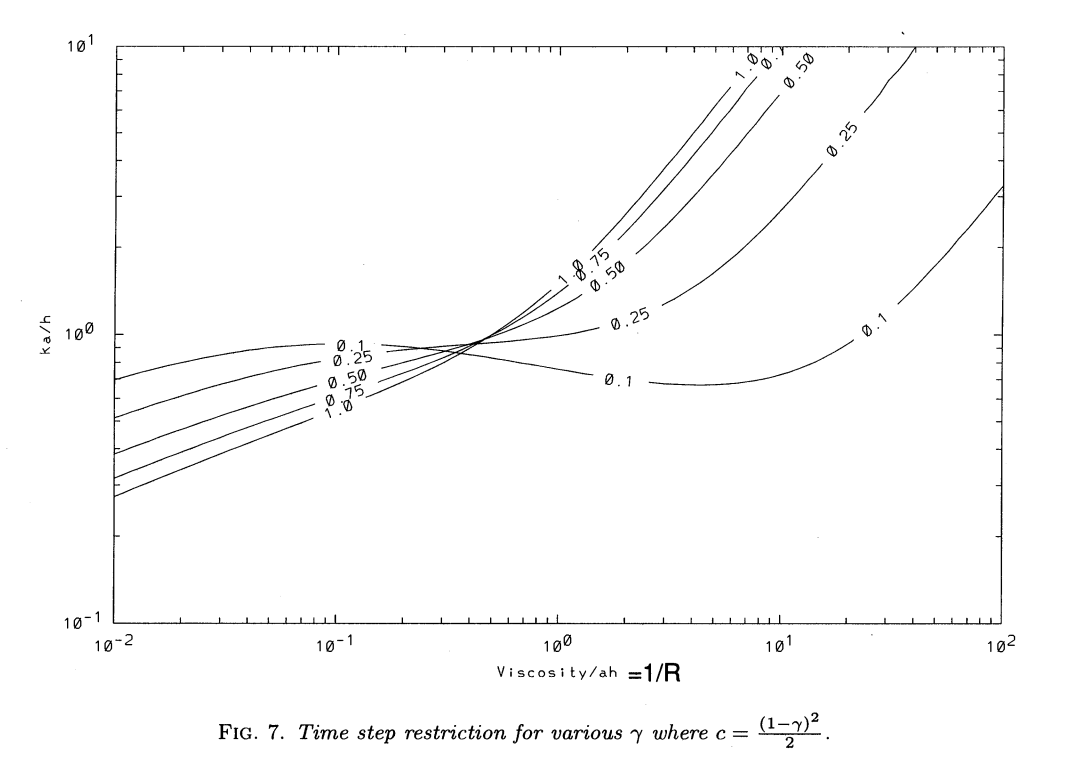
\includegraphics[scale=0.4]{./figures/Figure_3.png}
\end{figure}
\begin{figure}[H]
\centering
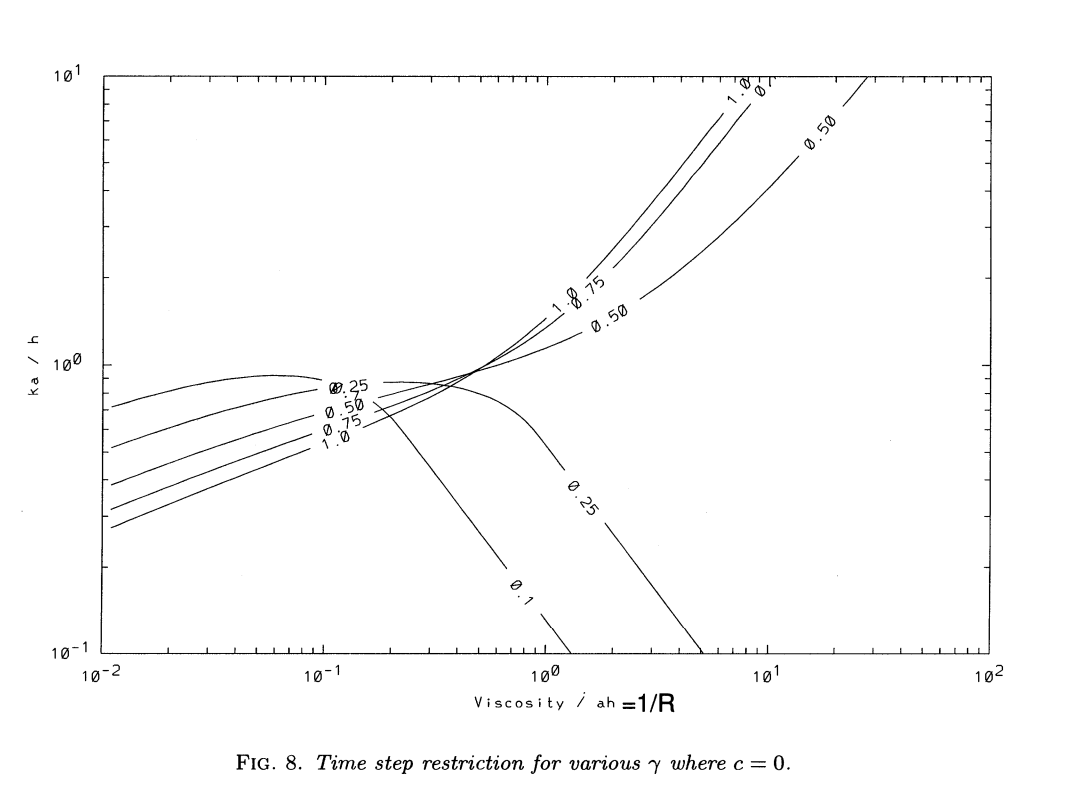
\includegraphics[scale=0.4]{./figures/Figure_4.png}
\end{figure}
\section{三阶隐式显式格式}
\begin{equation}
\begin{aligned}
\frac{1}{k}&\left[\left(\frac{1}{2}\gamma^2+\gamma+\frac{1}{3}+\theta\right)u^{n+1}+\left(\frac{3}{2}\gamma^2-2\gamma+\frac{1}{2}-\theta\right)u^n\right.\\
&\left.+\left(\frac{3}{2}\gamma^2+\gamma-1\right)u^{n-1}+\left(-\frac{1}{2}\gamma^2+\frac{1}{6}\right)u^{n-2}\right]\\
&=\left(\frac{\gamma^2+3\gamma}{2}+1+\frac{23}{12}\theta\right)f(u^n)-\left(\gamma^2+2\gamma+\frac{4}{3}\theta\right)f(u^{n-1})\\
&+\left(\frac{\gamma^2+\gamma}{2}+\frac{5}{12}\theta\right)f(u^{n-2})\\
&+\nu\left[\left(\frac{\gamma^2+\gamma}{2}+c\right)g(u^{n+1})+\left(1-\gamma^2-3c+\frac{23}{12}\theta\right)g(u^n)\right.\\
&\left.+\left(\frac{\gamma^2-\gamma}{2}+3c-\frac{4}{3}\theta\right)g(u^{n-1})+\left(\frac{5}{12}\theta-c\right)g(u^{n-2})\right]
\end{aligned}
\end{equation}
这些格式以时间步长$(n+\gamma)$到三阶。当$\theta=0$时对应于更低阶的格式,限制$0\le\gamma\le 1$为了防止大的截断误差。参数$c$通常乘以$\nu$,为了调整此参数以修正格式中$\nu$大的属性。
选择$(\gamma,\theta,c)=(1,0,0)$,我们将得到
\begin{equation}
\frac{1}{k}\left(\frac{11}{6}u^{n+1}-3u^n+\frac{3}{2}u^{n-1}-\frac{1}{3}u^{n-2}\right)=3f(u^n)-3f(u^{n-1})+f(u^{n-2})+\nu g(u^{n+1})
\end{equation}
这个格式隐式的部分采用了三阶的BDF,因此这个被称为三阶SBDF。
\section{四阶隐式显式格式}
对于$u'=f(u)+\nu g(u)$,这个格式由
\begin{equation}
\begin{aligned}
\frac{1}{k}&\left(\frac{25}{12}u^{n+1}-4u^n+3u^{n-1}-\frac{4}{3}u^{n-2}+\frac{1}{4}u^{n-3}\right)\\
&=4f(u^n)-6f(u^{n-1})+4f(u^{n-2})-f(u^{n-3})+\nu g(u^{n+1})
\end{aligned}
\end{equation}



\cite{tam19912d}
\bibliography{../../ref}
\end{document}













